\documentclass[12pt]{article}
%%%%%%%%%%%%%%%%
% Packages
%%%%%%%%%%%%%%%%

\usepackage[top=1.5cm,bottom=1.5cm,left=1.5cm,right= 1.5cm]{geometry}
\usepackage[parfill]{parskip}
\usepackage{graphicx, fontspec, xcolor,multicol, enumitem, setspace, amsmath, changepage}
\DeclareGraphicsRule{.tif}{png}{.png}{`convert #1 `dirname #1`/`basename #1 .tif`.png}

%%%%%%%%%%%%%%%%
% User defined colors
%%%%%%%%%%%%%%%%

% Pantone 2015 Fall colors
% http://iwork3.us/2015/02/18/pantone-2015-fall-fashion-report/
% update each semester or year

\xdefinecolor{custom_blue}{rgb}{0, 0.32, 0.48} % FROM SPRING 2016 COLOR PREVIEW
\xdefinecolor{custom_darkBlue}{rgb}{0.20, 0.20, 0.39} % Reflecting Pond  
\xdefinecolor{custom_orange}{rgb}{0.96, 0.57, 0.42} % Cadmium Orange
\xdefinecolor{custom_green}{rgb}{0, 0.47, 0.52} % Biscay Bay
\xdefinecolor{custom_red}{rgb}{0.58, 0.32, 0.32} % Marsala

\xdefinecolor{custom_lightGray}{rgb}{0.78, 0.80, 0.80} % Glacier Gray
\xdefinecolor{custom_darkGray}{rgb}{0.35, 0.39, 0.43} % Stormy Weather

%%%%%%%%%%%%%%%%
% Color text commands
%%%%%%%%%%%%%%%%

%orange
\newcommand{\orange}[1]{\textit{\textcolor{custom_orange}{#1}}}

% yellow
\newcommand{\yellow}[1]{\textit{\textcolor{yellow}{#1}}}

% blue
\newcommand{\blue}[1]{\textit{\textcolor{blue}{#1}}}

% green
\newcommand{\green}[1]{\textit{\textcolor{custom_green}{#1}}}

% red
\newcommand{\red}[1]{\textit{\textcolor{custom_red}{#1}}}

%%%%%%%%%%%%%%%%
% Coloring titles, links, etc.
%%%%%%%%%%%%%%%%

\usepackage{titlesec}
\titleformat{\section}
{\color{custom_blue}\normalfont\Large\bfseries}
{\color{custom_blue}\thesection}{1em}{}
\titleformat{\subsection}
{\color{custom_blue}\normalfont}
{\color{custom_blue}\thesubsection}{1em}{}

\newcommand{\ttl}[1]{ \textsc{{\LARGE \textbf{{\color{custom_blue} #1} } }}}

\newcommand{\tl}[1]{ \textsc{{\large \textbf{{\color{custom_blue} #1} } }}}

\usepackage[colorlinks=false,pdfborder={0 0 0},urlcolor= custom_orange,colorlinks=true,linkcolor= custom_orange, citecolor= custom_orange,backref=true]{hyperref}

%%%%%%%%%%%%%%%%
% Instructions box
%%%%%%%%%%%%%%%%

\newcommand{\inst}[1]{
\colorbox{custom_blue!20!white!50}{\parbox{\textwidth}{
	\vskip10pt
	\leftskip10pt \rightskip10pt
	#1
	\vskip10pt
}}
\vskip10pt
}

%%%%%%%%%%%
% App Ex number    %
%%%%%%%%%%%

% DON'T FORGET TO UPDATE

\newcommand{\appno}[1]
{1.2}

%%%%%%%%%%%%%%
% Turn on/off solutions      %
%%%%%%%%%%%%%%

% Off
%\newcommand{\soln}[2]{$\:$\\ \vspace{#1}}{}


%% On
\newcommand{\soln}[2]{\textit{\textcolor{custom_red}{#2}}}{}
\newcommand{\qt}[1]{\textcolor{custom_carnelian}{\textbf{#1.}}}
\newcommand{\qtq}[1]{\textcolor{custom_carnelian}{\textbf{#1?}}}
\newcommand{\ec}[1]{\textcolor{custom_carnelian}{\footnotesize{~(#1)}}}
%%%%%%%%%%%%%%%%
% Document
%%%%%%%%%%%%%%%%


%%%%% 1 %%%%%%%%%%%%%%%%%%%%%%%%%%%%%%%%%%%%%%%%%%%%%%%%%%%%%%%%%%%%%%%%%%%

\begin{document}
%fontspec[Ligatures=TeX]{Helvetica Neue Light}

Sergio I Garcia Rios \hfill GOVT 3990 Puzzle Solving with Data \\
Cornell University \hfill \\

\ttl{Midterm 1}

\inst{$\:$ \\
Name: \rule{10cm}{0.5pt} \\

Write your responses in the spaces provided below. \textbf{WRITE LEGIBLY and SHOW ALL WORK!}}

\qt{Marathon winners\label{marathon_winners}} The histogram and box plots below show the distribution of finishing times for male and female winners of the New York Marathon between 1970 and 1999.
\begin{center}
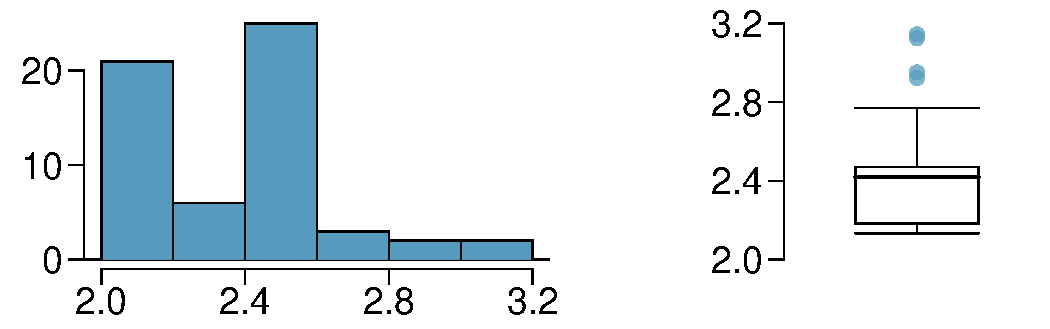
\includegraphics[width=0.6\textwidth]{figures/marathon_winners_hist_box.pdf}
\end{center}
\begin{enumerate}
\item What features of the distribution are apparent in the histogram and not the box plot? What features are apparent in the box plot but not in the histogram?
\vspace{2cm}


\item What may be the reason for the bimodal distribution? Explain.

\vspace{2cm}


\item Compare the distribution of marathon times for men and women based on the box plot shown below.

\begin{center}
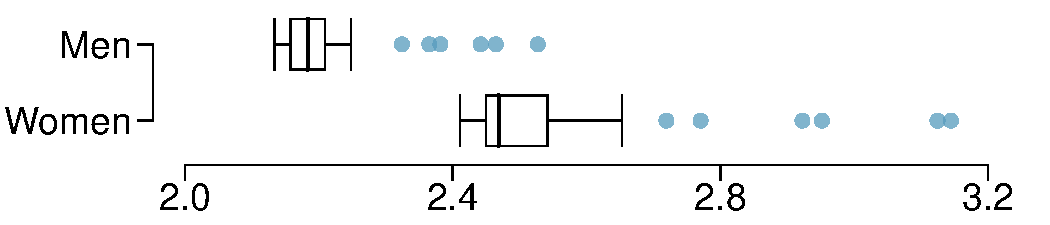
\includegraphics[width=0.6\textwidth]{figures/marathon_winners_gender_box.pdf}
\end{center}

\vspace{4cm}

\item The time series plot shown below is another way to look at these data. Describe what is visible in this plot but not in the others.
\vspace{2cm}

\end{enumerate}
\begin{center}
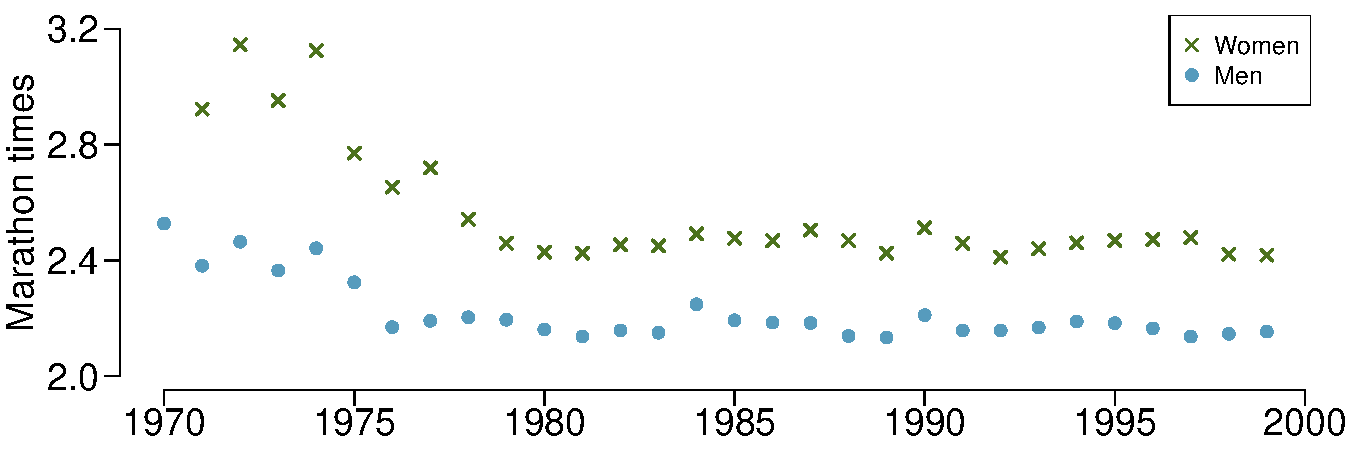
\includegraphics[width=0.75\textwidth]{figures/marathon_winners_time_series.pdf} \\
\end{center}
{}
\vspace{2cm}
%%%%% end %%%%%%%%%%%%%%%%%%%%%%%%%%%%%%%%%%%%%%%%%%%%%%%%%%%%%%%%%%%%%%%%%%%


%%%%% 1 %%%%%%%%%%%%%%%%%%%%%%%%%%%%%%%%%%%%%%%%%%%%%%%%%%%%%%%%%%%%%%%%%%%

\qt{Fisher's irises\label{fisher_irises}} Sir Ronald Aylmer Fisher was an 
English statistician, evolutionary biologist, and geneticist who worked on a 
data set that contained sepal length and width, and petal length and width from 
three species of iris flowers (\textit{setosa}, \textit{versicolor} and 
\textit{virginica}). There were 50 flowers from each species in the data set. 
%\footfullcite{Fisher:1936} \\

%\noindent\begin{minipage}[c]{0.48\textwidth}
\begin{enumerate}
\item How many cases were included in the data?
\vspace{.5cm}
\item How many numerical variables are included in the data? Indicate what 
they are, and if they are continuous or discrete.
\vspace{1cm}
\item How many categorical variables are included in the data, and what are 
they? List the corresponding levels (categories).
\vspace{2.5cm}
\end{enumerate}

\qt{Coin flips\label{coin_flips}} If you flip a fair coin 3 times, what is 
the probability of
\begin{enumerate}
\item getting all tails? 
\item getting all heads? 
\item getting at least one tails? 
\end{enumerate}
\clearpage
%%%%% end %%%%%%%%%%%%%%%%%%%%%%%%%%%%%%%%%%%%%%%%%%%%%%%%%%%%%%%%%%%%%%%%%%%

%%%%% 2 %%%%%%%%%%%%%%%%%%%%%%%%%%%%%%%%%%%%%%%%%%%%%%%%%%%%%%%%%%%%%%%%%%%

{\qt{Swing voters\label{swing_voters}} A 2012 Pew Research survey asked 2,373 
randomly sampled registered voters their political affiliation (Republican, 
Democrat, or Independent) and whether or not they identify as swing voters. 35\% 
of respondents identified as Independent, 23\% identified as swing voters, and 
11\% identified as both.
\begin{enumerate}
\item Are being Independent and being a swing voter disjoint, i.e. mutually 
exclusive?
\vspace{.5cm}
\item Draw a Venn diagram summarizing the variables and their associated 
probabilities.
\vspace{2.5cm}
\item What percent of voters are Independent but not swing voters?
\vspace{.5cm}
\item What percent of voters are Independent or swing voters?
\vspace{.5cm}
\item What percent of voters are neither Independent nor swing voters?
\vspace{.5cm}
\item Is the event that someone is a swing voter independent of the event that 
someone is a political Independent?
\vspace{1cm}
\end{enumerate}
}
%%%%% end %%%%%%%%%%%%%%%%%%%%%%%%%%%%%%%%%%%%%%%%%%%%%%%%%%%%%%%%%%%%%%%%%%%

%%%%% 3 %%%%%%%%%%%%%%%%%%%%%%%%%%%%%%%%%%%%%%%%%%%%%%%%%%%%%%%%%%%%%%%%%%%

\qt{Health coverage, frequencies\label{health_coverage_freqs}} The 
Behavioral Risk Factor Surveillance System (BRFSS) is an annual telephone survey 
designed to identify risk factors in the adult population and report emerging 
health trends. The following table summarizes two variables for the respondents: 
health status and health coverage, which describes whether each respondent had 
health insurance. 
\begin{center}
\begin{tabular}{rrrrrrrr}
                    &       & \multicolumn{5}{c}{\textit{Health Status}} &  \\ 
\cline{3-7}
                    &       & Excellent & Very good & Good  & Fair  & Poor  & Total\\ 
\cline{2-8}
\textit{Health}     & No    & 459       & 727       & 854   & 385   & 99    & 2,524 \\ 
\textit{Coverage}   & Yes   & 4,198     & 6,245     & 4,821 & 1,634 & 578   & 17,476 \\ 
\cline{2-8}
                    & Total & 4,657     & 6,972     & 5,675 & 2,019 & 677   & 20,000
\end{tabular}
\end{center}
\begin{enumerate}
\item If we draw one individual at random, what is the probability that the 
respondent has excellent health and doesn't have health coverage?

\vspace{1cm}
\item If we draw one individual at random, what is the probability that the 
respondent has excellent health or doesn't have health coverage?

\vspace{1cm}
\end{enumerate}
%%%%% end %%%%%%%%%%%%%%%%%%%%%%%%%%%%%%%%%%%%%%%%%%%%%%%%%%%%%%%%%%%%%%%%%%%
\clearpage


%%%%% 4 %%%%%%%%%%%%%%%%%%%%%%%%%%%%%%%%%%%%%%%%%%%%%%%%%%%%%%%%%%%%%%%%%%%

\qt{Exit poll\label{tree_exit_poll}} Edison Research gathered exit poll 
results from several sources for the Wisconsin recall election of Scott Walker. 
They found that 53\% of the respondents voted in favor of Scott Walker. 
Additionally, they estimated that of those who did vote in favor for Scott 
Walker, 37\% had a college degree, while 44\% of those who voted against Scott 
Walker had a college degree. Suppose we randomly sampled a person who 
participated in the exit poll and found that he had a college degree. What is the 
probability that he voted in favor of Scott Walker?
\vspace{1.5cm}
%%%%% end %%%%%%%%%%%%%%%%%%%%%%%%%%%%%%%%%%%%%%%%%%%%%%%%%%%%%%%%%%%%%%%%%%%



%%%%% 5 %%%%%%%%%%%%%%%%%%%%%%%%%%%%%%%%%%%%%%%%%%%%%%%%%%%%%%%%%%%%%%%%%%%


\qt{Male children\label{male_children}} While it is often assumed that the 
probabilities of having a boy or a girl are the same, the actual probability 
of having a boy is slightly higher at 0.51. Suppose a couple plans to have 3 
kids. 
\begin{enumerate}
\item Use the binomial model to calculate the probability that two of them 
will be boys.

\vspace{1cm}
\item Write out all possible orderings of 3 children, 2 of whom are boys. Use 
these scenarios to calculate the same probability from part (1) but using the 
addition rule for disjoint outcomes. Confirm that your answers from parts (1) 
and (2) match.

\vspace{3cm}
\end{enumerate}


\qt{Manufacturing workers\label{manufacturing_avg}}If 34\% of NY manufacturing workers make more than \$19/hr, what is the probability that in a random sample of 100 NY manufacturing workers less than 30\% make more than \$19/hr.

\soln{2cm}{
$p = 0.34$, $n = 100$ \\
S/F: checks \\
$\mu = 0.34 \times 100 = 34$ and $\sigma = \sqrt{100 \times 0.34 \times 0.66} = 4.74$ \\
$P \left( K < 30 \right) = P \left( Z < \frac{30 - 34}{4.74} \right) = P(Z < -0.84) = 0.2$
}



\clearpage

\qt{Manufacturing workers\label{manufacturing_avg}} Government data indicates that the average hourly wage for manufacturing workers in the United States is \$18.61, 
with a standard deviation of \$1.35. 

\begin{enumerate}

\item What Z score of manufacturing workers making more than \$20/hour?

\soln{3.5cm}{
Given: $X_{US} \sim N(\mu = 18.61, \sigma = 1.35)$
\[ P(X > 20) = P\left( Z > \frac{20 - 18.61}{1.35} \right) = P(Z > 1.02) = 0.154 \rightarrow 15.4\% \]
}


\item Using the \textit{Z-table} provided find the area under the bell curve to the left of z. \textit{For instance: For a value of $Z = 2.03$ we would say that .9788 fall under the curve or 97.88\% of the data.} 
\vspace{3cm}
\item With that information, assess whether the amount of hourly worker making more than \$20 is high or low. 
\end{enumerate}
\vspace{3cm}
%
%\item What percent of manufacturing workers make between \$18 - \$20/hour? \\
%
%\soln{3.5cm}{
%\[ P(X_{US} > 18) = P\left( Z > \frac{18 - 18.61}{1.35} \right) = P(Z > -0.45) = 0.674 \]
%\[ P(18 < X_{US} < 20) = 0.674 - 0.154 = 0.52 \rightarrow 52\% \]
%}
%
%\clearpage
\qt{R functions} Looking at the following \texttt{R} function and given that $x = 17$ 
\begin{verbatim}
function(x){
  if(!is.atomic(x)){x <- x[,1]}
  y <- rep(0,length(x))
  y[x == "H"] <- 1
  y <- c(0, y, 0)
  wz <- which(y == 0)
  streak <- diff(wz) - 1
  return(data.frame(length = streak))
}
\end{verbatim}

\begin{enumerate}
\item What would be the last item in the iteration?
\end{enumerate}


\end{document}